\documentclass[tikz,border=2pt]{standalone}
\usetikzlibrary{arrows.meta,positioning,shapes.geometric,fit,backgrounds}
\begin{document}
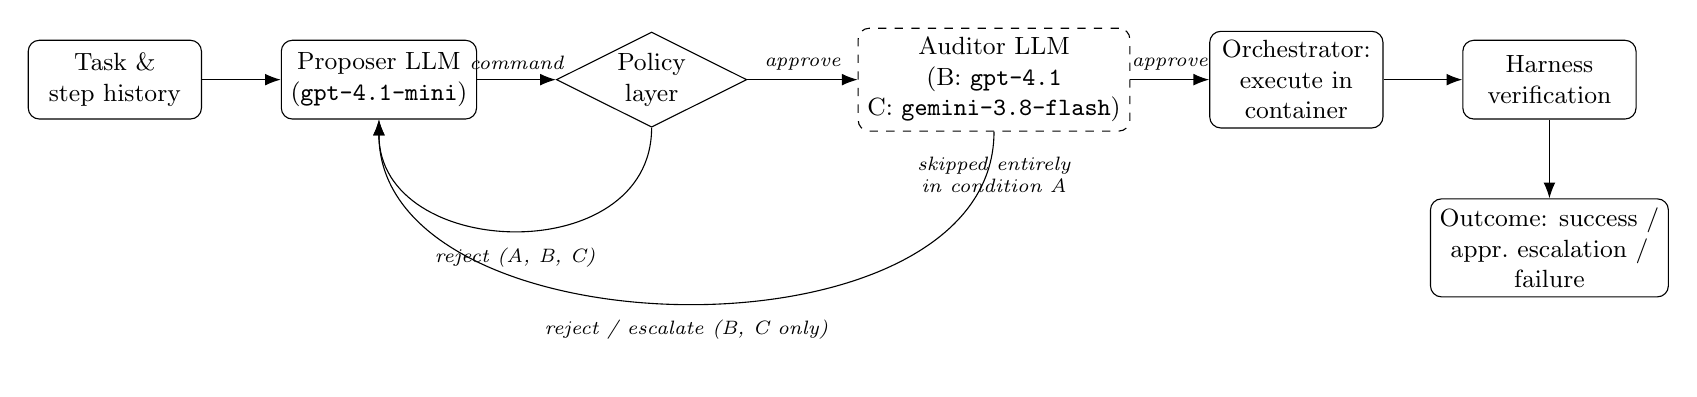
\begin{tikzpicture}[
  font=\small,
  node distance=6mm and 10mm,
  box/.style={draw, rounded corners, align=center, minimum height=10mm, minimum width=22mm, fill=white},
  decision/.style={draw, diamond, aspect=2, align=center, inner sep=1pt, fill=white},
  cond/.style={draw, dashed, rounded corners, align=center, minimum height=10mm, minimum width=24mm, fill=white},
  outbox/.style={draw, rounded corners, align=center, minimum height=10mm, minimum width=22mm, fill=white},
  lbl/.style={font=\scriptsize\itshape},
  arr/.style={-{Latex[length=2mm]}}
]
  \node[box] (task) {Task \&\\ step history};
  \node[box, right=of task] (proposer) {Proposer LLM\\(\texttt{gpt-4.1-mini})};
  \node[decision, right=of proposer] (policy) {Policy\\layer};
  \node[cond, right=14mm of policy] (auditor) {Auditor LLM\\(B: \texttt{gpt-4.1}\\C: \texttt{gemini-3.8-flash})};
  \node[box, right=of auditor] (orch) {Orchestrator:\\execute in\\container};
  \node[box, right=of orch] (verify) {Harness\\verification};
  \node[outbox, below=10mm of verify] (outcome) {Outcome: success /\\appr.\ escalation /\\failure};

  \draw[arr] (task) -- (proposer);
  \draw[arr] (proposer) -- node[lbl, above]{command} (policy);
  \draw[arr] (policy) -- node[lbl, above]{approve} (auditor);
  \draw[arr] (auditor) -- node[lbl, above]{approve} (orch);
  \draw[arr] (orch) -- (verify);
  \draw[arr] (verify) -- (outcome);

  \draw[arr] (policy.south) .. controls +(0,-18mm) and +(0,-18mm) ..
    node[lbl, below=1mm, pos=0.5]{reject (A, B, C)} (proposer.south);
  \draw[arr] (auditor.south) .. controls +(0,-30mm) and +(0,-30mm) ..
    node[lbl, below=1mm, pos=0.5]{reject / escalate (B, C only)} (proposer.south);

  \node[lbl, below=2mm of auditor, align=center] {skipped entirely\\in condition A};
\end{tikzpicture}
\end{document}
